%%%%%%%%%%%%%%%%%%%%%%%%%%%%%%%%%%%%%%%%%
% Beamer Presentation
% LaTeX Template
% Version 1.0 (10/11/12)
%
% This template has been downloaded from:
% http://www.LaTeXTemplates.com
%
% License:
% CC BY-NC-SA 3.0 (http://creativecommons.org/licenses/by-nc-sa/3.0/)
%
%%%%%%%%%%%%%%%%%%%%%%%%%%%%%%%%%%%%%%%%%

%----------------------------------------------------------------------------------------
%	PACKAGES AND THEMES
%----------------------------------------------------------------------------------------

\documentclass{beamer}

\mode<presentation> {

% The Beamer class comes with a number of default slide themes
% which change the colors and layouts of slides. Below this is a list
% of all the themes, uncomment each in turn to see what they look like.

%\usetheme{default}
%\usetheme{AnnArbor}
%\usetheme{Antibes}
%\usetheme{Bergen}
%\usetheme{Berkeley}
%\usetheme{Berlin}
%\usetheme{Boadilla}
%\usetheme{CambridgeUS}
%\usetheme{Copenhagen}
%\usetheme{Darmstadt}
%\usetheme{Dresden}
%\usetheme{Frankfurt}
%\usetheme{Goettingen}
%\usetheme{Hannover}
%\usetheme{Ilmenau}
%\usetheme{JuanLesPins}
%\usetheme{Luebeck}
\usetheme{Madrid}
%\usetheme{Malmoe}
%\usetheme{Marburg}
%\usetheme{Montpellier}
%\usetheme{PaloAlto}
%\usetheme{Pittsburgh}
%\usetheme{Rochester}
%\usetheme{Singapore}
%\usetheme{Szeged}
%\usetheme{Warsaw}

% As well as themes, the Beamer class has a number of color themes
% for any slide theme. Uncomment each of these in turn to see how it
% changes the colors of your current slide theme.

%\usecolortheme{albatross}
%\usecolortheme{beaver}
%\usecolortheme{beetle}
%\usecolortheme{crane}
%\usecolortheme{dolphin}
%\usecolortheme{dove}
%\usecolortheme{fly}
%\usecolortheme{lily}
%\usecolortheme{orchid}
%\usecolortheme{rose}
%\usecolortheme{seagull}
%\usecolortheme{seahorse}
%\usecolortheme{whale}
%\usecolortheme{wolverine}

%\setbeamertemplate{footline} % To remove the footer line in all slides uncomment this line
%\setbeamertemplate{footline}[page number] % To replace the footer line in all slides with a simple slide count uncomment this line

%\setbeamertemplate{navigation symbols}{} % To remove the navigation symbols from the bottom of all slides uncomment this line
}
\graphicspath{{Images/}}
\usepackage{graphicx} % Allows including images
\usepackage{booktabs} % Allows the use of \toprule, \midrule and \bottomrule in tables

\usepackage[utf8]{inputenc}% A modifier en fonction du codage d'entrée
\usepackage[T1]{fontenc}
\usepackage{lmodern}% Ou autre fonte

 \usepackage[french]{babel}
%----------------------------------------------------------------------------------------
%	TITLE PAGE
%----------------------------------------------------------------------------------------

\title[Magic Tiles]{Soutenance de Projet : Développement Mobile} % The short title appears at the bottom of every slide, the full title is only on the title page

\author{Kamarouzamane Combo \& Hajanirina Randimbisoa} % Your name

\institute{\normalsize{M1 Informatique Université de la Réunion}}

\date{\today} % Date, can be changed to a custom date

\begin{document}

\begin{frame}
\titlepage % Print the title page as the first slide
\end{frame}

\begin{frame}
\frametitle{Sommaire} % Table of contents slide, comment this block out to remove it
\tableofcontents % Throughout your presentation, if you choose to use \section{} and \subsection{} commands, these will automatically be printed on this slide as an overview of your presentation
\end{frame}

%----------------------------------------------------------------------------------------
%	PRESENTATION SLIDES
%----------------------------------------------------------------------------------------

%-------------------------------------------------------------------------------------------------------------------------------------------------------------
\section{Introduction}
%-------------------------------------------------------------------------------------------------------------------------------------------------------------

%\subsection{Subsection Example} % A subsection can be created just before a set of slides with a common theme to further break down your presentation into chunks


\begin{frame}
  \frametitle{Introduction}
  \begin{block}{Objectif}
    \begin{itemize}
    \item {Créer une application mobile sur Android et iOS}
    \end{itemize}
  \end{block}
    \begin{block}{Contraintes}
    \begin{itemize}
    \item {Changement de configuration}
    \item {Géolocalisation}
    \item {Utiliser un capteur}
    \item {Utilisation d' au moins un geste courant non-trivial}
    \item {Ajouter du son}
    \end{itemize}
  \end{block}
\end{frame}


%-------------------------------------------------------------------------------------------------------------------------------------------------------------
\section{Présentation du jeu}
%-------------------------------------------------------------------------------------------------------------------------------------------------------------

\begin{frame}
  \frametitle{Présentation du jeu}
\begin{block}{Principe} 
    \begin{itemize}
         \item {Le jeu Magic Tiles est un jeu de modélisation et de simulation des touches de piano}
     \begin{center}
      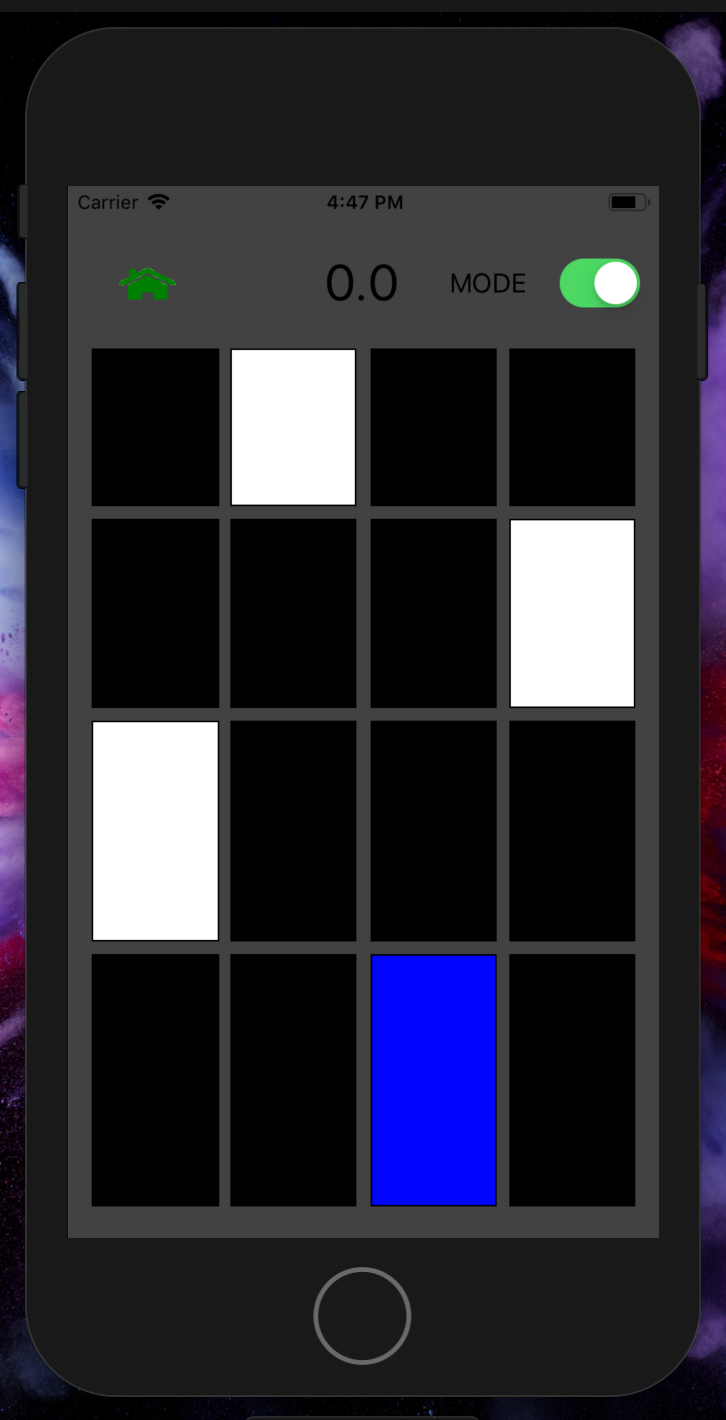
\includegraphics[width=20mm]{iOSapp1}
      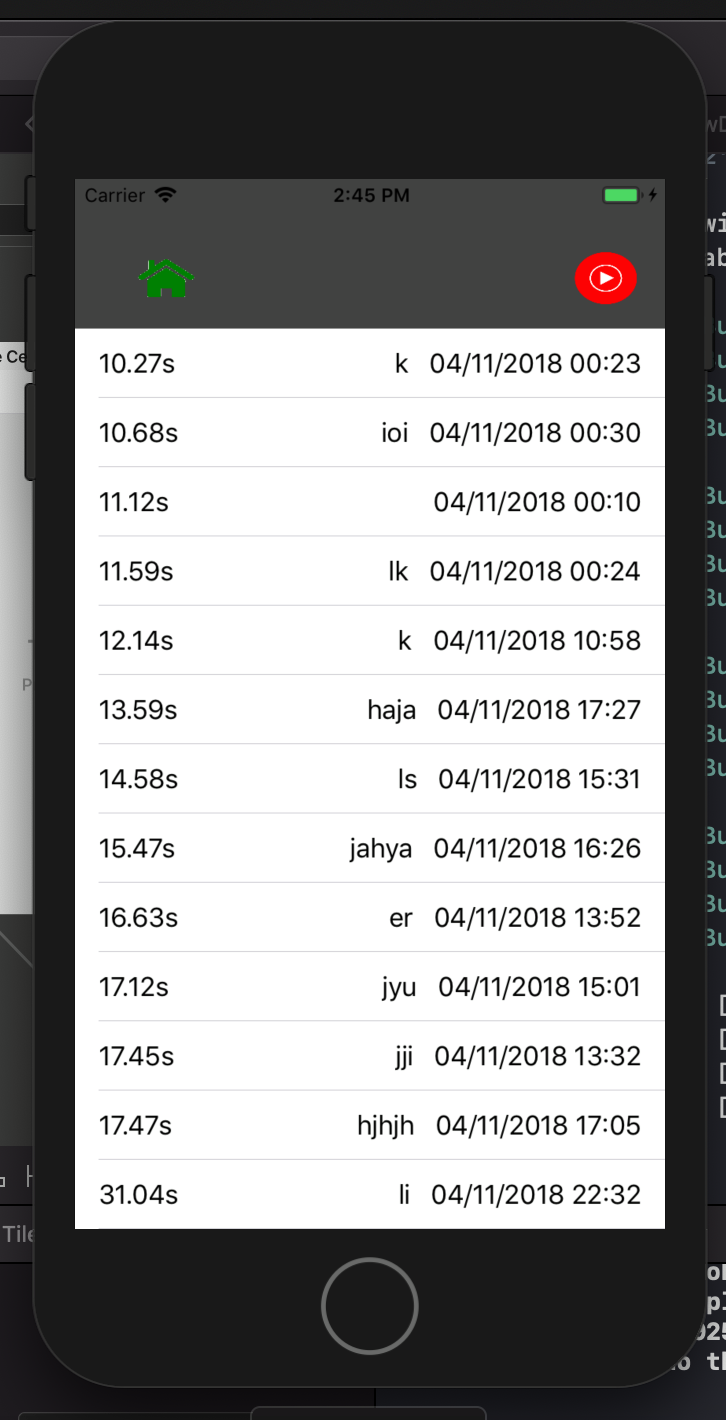
\includegraphics[width=20mm]{iOS}

    \end{center}
    \end{itemize}
  \end{block}

\end{frame}

%---------------------------------------------------------------------------------------------------------------------------------------------------------
\section{Android}
%---------------------------------------------------------------------------------------------------------------------------------------------------------

\begin{frame}
\frametitle{Android}
\begin{block}{Présentation}
% Your image included here
\end{block}

\end{frame}

%------------------------------------------------
\begin{frame}
\begin{block}{Portion de code}
\end{block}
   
\end{frame}



%---------------------------------------------------------------------------------------------------------------------------------------------------------
\section{iOS}
%---------------------------------------------------------------------------------------------------------------------------------------------------------
   
\begin{frame}
\frametitle{iOS}
 \begin{block}{Création de l'application : }
    \begin{itemize}
    \item {Quand on crée un nouveau projet, plusieurs options nous sont offertes. Le premier sert à effectuer des tests (Playgrounds) de code swift pour déboguer sans démarrer de véritable projet. Le deuxième permet de créer un nouveau véritable projet. Le troisième sert si vous avez un repository à votre dispotition sur un git, il est alors possible de le récupérer ainsi.}
    \end{itemize}
  \end{block}

	\begin{block}{Storyboard et programmation  : MVC}
	\par La structure de projet iOS est basée sur le modèle MVC ( Modèle Vue Controlleur)
	 \begin{itemize}
    	\item {Modèle: Les données de l’applications }
	\item {Vue: La partie visuelle de l’application, c’est en quelque sorte l’IHM  }
	\item {Controlleur: Contrôleur, c’est la partie logique de notre application, elle va permettre d’interagir entre les différentes vues }
 
    \end{itemize}
	\end{block}
\end{frame}

\begin{frame}
\frametitle{iOS}
\begin{block}{Storyboard et programmation }
		 \begin{itemize}
\item {Accueil:  contenant les fonctionnalités de l'application} 
    	\item {AnimationButton.swift: création d'une animation sur les bouttons }
   	 \item {AppDelegate.swift : gère les événements du cycle de vie d'une application}
 	  \item {Camera.swift: l'appareil photo}	
  	  \item {Game.swift : présenter à l'aide d'un boutton play en rouge}
	 \item {Highscores.swift : historique des scores sauvegardés }
	    \item {Localisation.swift: permet de faire une  géolocalisation}
	    \item {Save.swift : sauvegarde des temps mis pour le jeux}
	    \item {ViewController.swift : corps de l'application}
  \end{itemize}
	\end{block}

\end{frame}


\begin{frame}
	\frametitle{iOS}
	\begin{block}{Storyboard et programmation}
	\par Pour en conclure avec cela, les fichiers AppDelegate.swift et Main.swift sont donc les code sources des contrôleurs de notre application. Les fichiers .storyboard sont les vues de l’application (LaunchScreen pour l’écran de démarrage d’une application, et Main pour la première vue de l’application)
	\end{block}
\end{frame}


\begin{frame}
\frametitle{iOS}
	\frametitle{iOS}
	\begin{block}{Explication d'autre méthodes}
	 \begin{itemize}
	\item {ViewDidLoad :  appelée automatiquement lorsque la vue se charge } 
    	\item {didRecieveMemoryWarning:appelée lorsque l’iPhone est surchargé en mémoire vive (RAM), c’est donc pour permettre une bonne optimisation et donc éviter que l’application ne crash.}
\item {@NSManaged :  permet à Xcode de faire le lien avec l'attribut de notre entité } 
\item {CoreData :  permet d'utiliser les classes qui s'y rapportent } 
 	
  \end{itemize}
	\end{block}
\end{frame}

%---------------------------------------------------------------------------------------------------------------------------------------------------------
\section{Démonstration}
%---------------------------------------------------------------------------------------------------------------------------------------------------------

\begin{frame}
\frametitle{Démonstration}
	\Huge{\centerline{Démonstration}}
\end{frame}

%---------------------------------------------------------------------------------------------------------------------------------------------------------
\section{Conclusion}
%---------------------------------------------------------------------------------------------------------------------------------------------------------


\begin{frame}
\frametitle{Conclusion}
	\Huge{\centerline{Conclusion}}
	Ce projet a fait l'objet d'une expérience à  la fois intéressante et enrichissante, qui nous a permis d'améliorer nos connaissances et nos compétences dans le domaine du développement d'applications mobile.
\end{frame}

\begin{frame}
\Huge{\centerline{The End}}
\end{frame}

%----------------------------------------------------------------------------------------

\end{document} 